\documentclass{article}
\usepackage[utf8]{inputenc}
\usepackage{amsmath, amssymb}
\usepackage{mathtools}
\usepackage{a4wide}
\usepackage{appendix}
\usepackage{listings}
\usepackage{float}
\usepackage{subcaption}
\usepackage{hyperref}
\usepackage{float}
\usepackage{qtree}
\usepackage[usenames,dvipsnames]{xcolor}
\usepackage{color}
\usepackage{tikz}
\usepackage{pgfplots}
\pgfplotsset{compat=1.16}
\usepackage{caption}
\usepackage[top=2cm, bottom=2cm]{geometry}


\newcommand\scalemath[2]{\scalebox{#1}{\mbox{\ensuremath{\displaystyle #2}}}}


\definecolor{codegreen}{rgb}{0,0.6,0}
\definecolor{codegray}{rgb}{0.5,0.5,0.5}
\definecolor{codepurple}{rgb}{0.58,0,0.82}
\definecolor{backcolour}{rgb}{0.95,0.95,0.92}

\lstdefinestyle{mystyle}{
    backgroundcolor=\color{backcolour},   
    commentstyle=\color{codegreen},
    keywordstyle=\color{magenta},
    numberstyle=\tiny\color{codegray},
    stringstyle=\color{codepurple},
    basicstyle=\ttfamily\footnotesize,
    breakatwhitespace=false,         
    breaklines=true,                 
    captionpos=b,                    
    keepspaces=true,                 
    numbers=left,                    
    numbersep=5pt,                  
    showspaces=false,                
    showstringspaces=false,
    showtabs=false,                  
    tabsize=2
}

\lstset{style=mystyle}

\newcommand{\diff}[2]{\frac{\text{d} #1}{\text{d} #2}}

\title{
    Look inside the forest \\
    \large X-ray and Computed Tomography
}
\author{Hugo M. Nielsen (s214734) \and Mikael H. Hoffmann (s214753) \and Christian Valentin Kjær (s211469) \and Jacob Tuxen (s194572)}
\date{7/5-2023}

\begin{document}
\maketitle



\newpage

% ASSUMPTIONS
%% Mean is normally distributed with mean = 0
%% Tree is homogoen

\section{Problem and background} 
Due to hunting in forrests, shots are often found embedded in logs. This can impede the work of wood processing plants, as steel shots can discolour the wood and damage the saw blades. Therefore, one such plant, has reached out to us for guidance on designing a CT-scanner that can detect these shots before cutting the wood. \\
As CT-scanners are expensive to operate, the wood processing company would like to use as few angles and as few rays as possible for the CT-scanner while also minimizing the time, the model takes to reconstruct the image.


\section{Data and experiments}
\subsection{Data - simulations}
CT-scanners allow us to look inside objects, without cutting them open, by computing attenuation distributions over every angle used in the model and reconstruct the attenuation coefficients of the material from these distributions. This let's us identify compounds using the known attenuation coefficients of compounds we expect might be inside the object. \\ 
How representative these distributions are of the actual object depends on the number of rays used by the CT-scanner, the number of angles, corresponding to the number of unique distributions, and the resolution used for the image. This is illustrated here for two orthogonal angles:

% Kan man kigge på den her figur og vide hvad den visualisere på 3 sekunder? Hvordan kan den forbedres? 
\begin{figure}[htbp]
    \centering
\large{CT-scanner output distributions} \\
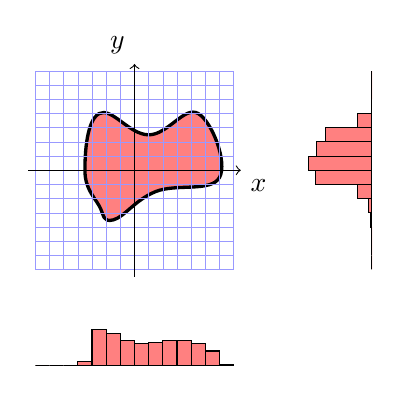
\begin{tikzpicture}[scale=0.9]
  % Draw blob
  \draw [very thick, fill=red!50] plot [smooth cycle,tension=0.7] coordinates {(-0.3,-0.7) (0.3,-0.3) (1.2,-0.1) (0.9,0.8) (0.2,0.5) (-0.5,0.8) (-0.7,0) (-0.5,-0.5)};
  
  % Draw grid
  \draw [step=0.2cm,blue!40,very thin] (-1.4,-1.4) grid (1.4,1.4);
  
  % Draw axes
  \draw [->] (-1.5,0) -- (1.5,0) node [below right] {$x$};
  \draw [->] (0,-1.5) -- (0,1.5) node [above left] {$y$};
  
  % Barplot
  \begin{scope}[shift={(3.35,0)},rotate=90]
      \draw [fill=red!50] (-1.4,0) rectangle (-1.4+0.2, 0);
      \draw [fill=red!50] (-1.2,0) rectangle (-1.2+0.2, 0);      \draw [fill=red!50] (-1.0,0) rectangle (-1.0+0.2, 0); \draw [fill=red!50] (-0.8,0) rectangle (-0.8+0.2, 0.0125);\draw [fill=red!50] (-0.6,0) rectangle (-0.6+0.2, 0.05);\draw [fill=red!50] (-0.4,0) rectangle (-0.4+0.2, 0.2);\draw [fill=red!50] (-0.2,0) rectangle (-0.2+0.2, 0.8);\draw [fill=red!50] (0,0) rectangle (0+0.2, 0.9);\draw [fill=red!50] (0.2,0) rectangle (0.2+0.2, 0.78);\draw [fill=red!50] (0.4,0) rectangle (0.4+0.2, 0.65);\draw [fill=red!50] (0.6,0) rectangle (0.6+0.2, 0.2);\draw [fill=red!50] (0.8,0) rectangle (0.8+0.2, 0.01);\draw [fill=red!50] (1.0,0) rectangle (1.0+0.2, 0);\draw [fill=red!50] (1.2,0) rectangle (1.2+0.2, 0);
  \end{scope}

    % Barplot Bottom
  \begin{scope}[shift={(0,-2.75)}]
      \draw [fill=red!50] (-1.4,0) rectangle (-1.4+0.2, 0);
      \draw [fill=red!50] (-1.2,0) rectangle (-1.2+0.2, 0);      \draw [fill=red!50] (-1.0,0) rectangle (-1.0+0.2, 0); \draw [fill=red!50] (-0.8,0) rectangle (-0.8+0.2, 0.05);\draw [fill=red!50] (-0.6,0) rectangle (-0.6+0.2, 0.5);\draw [fill=red!50] (-0.4,0) rectangle (-0.4+0.2, 0.45);\draw [fill=red!50] (-0.2,0) rectangle (-0.2+0.2, 0.35);\draw [fill=red!50] (0,0) rectangle (0+0.2, 0.3);\draw [fill=red!50] (0.2,0) rectangle (0.2+0.2, 0.32);\draw [fill=red!50] (0.4,0) rectangle (0.4+0.2, 0.35);\draw [fill=red!50] (0.6,0) rectangle (0.6+0.2, 0.35);\draw [fill=red!50] (0.8,0) rectangle (0.8+0.2, 0.3);\draw [fill=red!50] (1.0,0) rectangle (1.0+0.2, 0.2);\draw [fill=red!50] (1.2,0) rectangle (1.2+0.2, 0.01);
  \end{scope}
\end{tikzpicture} \hfill
% Bad resolution
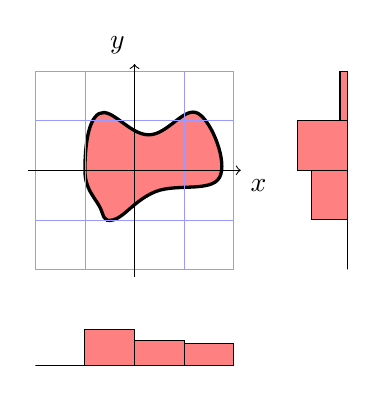
\begin{tikzpicture}[scale=0.9]
% Draw blob
\draw [very thick, fill=red!50] plot [smooth cycle,tension=0.7] coordinates {(-0.3,-0.7) (0.3,-0.3) (1.2,-0.1) (0.9,0.8) (0.2,0.5) (-0.5,0.8) (-0.7,0) (-0.5,-0.5)};

% Draw grid
\draw [step=0.699cm,blue!40,very thin] (-1.4,-1.4) grid (1.4,1.4);

% Draw axes
\draw [->] (-1.5,0) -- (1.5,0) node [below right] {$x$};
\draw [->] (0,-1.5) -- (0,1.5) node [above left] {$y$};

% Barplot (bottom)
  \begin{scope}[shift={(0,-2.75)}]
      \draw [fill=red!50] (-1.4,0) rectangle (-1.4+0.7, 0);
      \draw [fill=red!50] (-0.7,0) rectangle (-1.4+1.4, 0.5);
      \draw [fill=red!50] (0,0) rectangle (-1.4+2.1, 0.35);
      \draw [fill=red!50] (0.7,0) rectangle (-1.4+2.8, 0.3);
  \end{scope}

% Barplot (right)
\begin{scope}[shift={(3,0)},rotate=90]
      \draw [fill=red!50] (-1.4,0) rectangle (-1.4+0.7, 0);
      \draw [fill=red!50] (-0.7,0) rectangle (-1.4+1.4, 0.5);
      \draw [fill=red!50] (0,0) rectangle (-1.4+2.1, 0.7);
      \draw [fill=red!50] (0.7,0) rectangle (-1.4+2.8, 0.1);
\end{scope}
\end{tikzpicture} \hfill
% Few rays
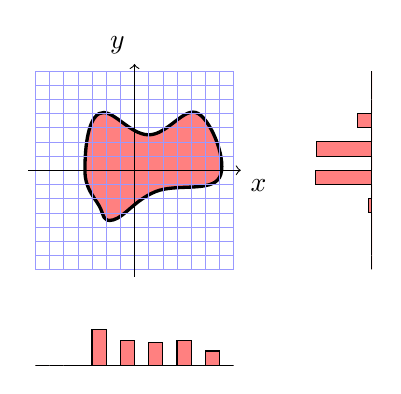
\begin{tikzpicture}[scale=0.9]
  % Draw blob
  \draw [very thick, fill=red!50] plot [smooth cycle,tension=0.7] coordinates {(-0.3,-0.7) (0.3,-0.3) (1.2,-0.1) (0.9,0.8) (0.2,0.5) (-0.5,0.8) (-0.7,0) (-0.5,-0.5)};
  
  % Draw grid
  \draw [step=0.2cm,blue!40,very thin] (-1.4,-1.4) grid (1.4,1.4);
  
  % Draw axes
  \draw [->] (-1.5,0) -- (1.5,0) node [below right] {$x$};
  \draw [->] (0,-1.5) -- (0,1.5) node [above left] {$y$};
  
  % Barplot
  \begin{scope}[shift={(3.35,0)},rotate=90]
      \draw [fill=red!50] (-1.4,0) rectangle (-1.4+0.2, 0);
      \draw [fill=red!50] (-1.2,0) rectangle (-1.2+0.2, 0);      \draw [fill=red!50] (-1.0,0) rectangle (-1.0+0.2, 0); \draw [fill=red!50] (-0.8,0) rectangle (-0.8+0.2, 0);\draw [fill=red!50] (-0.6,0) rectangle (-0.6+0.2, 0.05);\draw [fill=red!50] (-0.4,0) rectangle (-0.4+0.2, 0);\draw [fill=red!50] (-0.2,0) rectangle (-0.2+0.2, 0.8);\draw [fill=red!50] (0,0) rectangle (0+0.2, 0);\draw [fill=red!50] (0.2,0) rectangle (0.2+0.2, 0.78);\draw [fill=red!50] (0.4,0) rectangle (0.4+0.2, 0);\draw [fill=red!50] (0.6,0) rectangle (0.6+0.2, 0.2);\draw [fill=red!50] (0.8,0) rectangle (0.8+0.2, 0);\draw [fill=red!50] (1.0,0) rectangle (1.0+0.2, 0);\draw [fill=red!50] (1.2,0) rectangle (1.2+0.2, 0);
  \end{scope}

    % Barplot Bottom
  \begin{scope}[shift={(0,-2.75)}]
      \draw [fill=red!50] (-1.4,0) rectangle (-1.4+0.2, 0);
      \draw [fill=red!50] (-1.2,0) rectangle (-1.2+0.2, 0);      \draw [fill=red!50] (-1.0,0) rectangle (-1.0+0.2, 0); \draw [fill=red!50] (-0.8,0) rectangle (-0.8+0.2, 0);\draw [fill=red!50] (-0.6,0) rectangle (-0.6+0.2, 0.5);\draw [fill=red!50] (-0.4,0) rectangle (-0.4+0.2, 0);\draw [fill=red!50] (-0.2,0) rectangle (-0.2+0.2, 0.35);\draw [fill=red!50] (0,0) rectangle (0+0.2, 0);\draw [fill=red!50] (0.2,0) rectangle (0.2+0.2, 0.32);\draw [fill=red!50] (0.4,0) rectangle (0.4+0.2, 0);\draw [fill=red!50] (0.6,0) rectangle (0.6+0.2, 0.35);\draw [fill=red!50] (0.8,0) rectangle (0.8+0.2, 0);\draw [fill=red!50] (1.0,0) rectangle (1.0+0.2, 0.2);\draw [fill=red!50] (1.2,0) rectangle (1.2+0.2, 0);
  \end{scope}
\end{tikzpicture}
    \captionsetup{justification=centering}
    \caption[]{\small Illustration of the output of a CT scanner from two orthogonal angles, using different resolutions and number of rays. \emph{Leftmost:} many rays, good resolution. \emph{Center:} few rays, bad resolution. \emph{Rightmost:} few rays, good resolution}
    \label{fig:tikz-pictures}
\end{figure} 
Therefore, as part of constructing a fast and costefficient CT-scanner design, we simulate distributions using different numbers of rays and angles, and at different resolutions for use in determinening the best combination of these parameters. Moreover, we want our parameters to be robust towards noise and to different possible wood-shapes and shot-distributions and thus also simulate distributions varying these parameters.

\subsection{Data - attenuation coefficients} \label{NISTDATA}
From NIST\footnote{See \url{https://www.nist.gov/pml/x-ray-mass-attenuation-coefficients}.} we collected the attenuation coefficients for iron/steel, lead, bismuth and wood\footnote{The attenuation coefficients for wood were calculated based on its percentagewise composition of carbon, hydrogen and oxygen - based on the source: ???.}. Based on the 


\section{Mathematical model}
\subsection{CT - attenuation distributions - discretization}
The goal is to reconstruct the object image from the attenuation distributions obtained from the CT-scanner. To that end we first need to understand, how a CT-scanner constructs the attenuation distributions and for that we need Lambert Beer's law. Lambert Beer's law let's us relate the attenuation of every point on a CT-scanner ray to a point in the CT-scanner output distribution in terms of a line integral\footnote{Lambert Beer's law is often stated in terms of an equivalent differential equation, see appendix \ref{appendix:lambert-beers-law}.}: \\
\begin{equation}
    \int_{0}^{\ell_{\max}}x \text{d} \ell = \log\left(\frac{I_0}{I}\right)
\end{equation}
Where the integration interval $[0, \ell_{\max}]$ is of the ray over the object of interest, $x$ the material dependant attenuation coefficient for every point along the ray through the material and $\log\left(\frac{I_0}{I}\right)$ the value of the point on the attenuation distribution i.e. the attenuation over the whole line. \\
Solving this setup is, however, very complicated and we therefore make the simplification, that we can approximate the object as a finite number of homogeneous pixels\footnote{Homogeneous in terms of attenuation coefficients.}. \\
\begin{figure}[htbp]
    \centering
\large{Discretization of model} \\
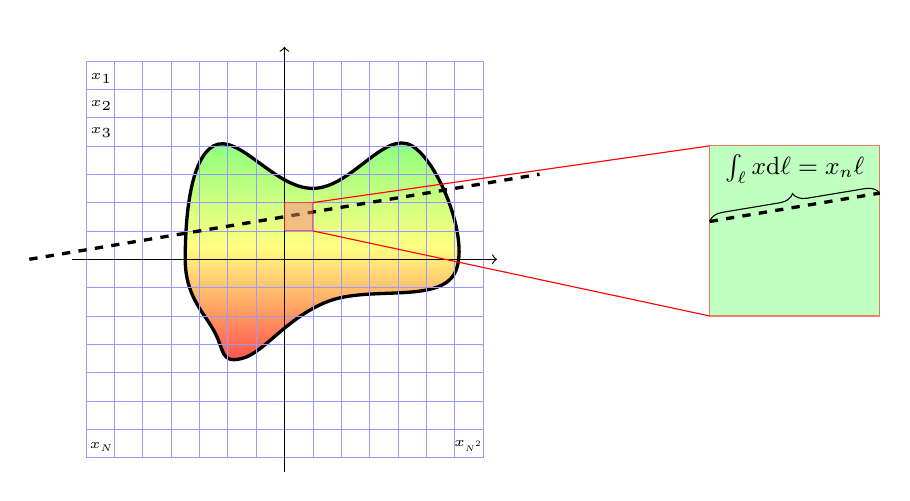
\begin{tikzpicture}[scale=1.8]
% Define color gradient
\pgfdeclareverticalshading{blobgrad}{100bp}{
color(0bp)=(red!70);
color(25bp)=(red!70);
color(50bp)=(yellow!50);
color(75bp)=(green!50);
color(100bp)=(blue!50)
}
% Draw blob with color gradient
\shadedraw [very thick, shading=blobgrad] plot [smooth cycle,tension=0.7] coordinates {(-0.3,-0.7) (0.3,-0.3) (1.2,-0.1) (0.9,0.8) (0.2,0.5) (-0.5,0.8) (-0.7,0) (-0.5,-0.5)};
% Draw grid
\draw [step=0.2cm,blue!40,very thin] (-1.4,-1.4) grid (1.4,1.4);
% Draw axes
\draw [->] (-1.5,0) -- (1.5,0) node [below right] {};
\draw [->] (0,-1.5) -- (0,1.5) node [above left] {};

% Draw slanted line
\draw [very thick, dashed] (-1.8,0) coordinate (start) -- (1.8,0.6) coordinate (end);

% Draw zoombox lines
\draw [color=red] (0.2, 0.2) -- (3,-0.4);
\draw [color=red] (0.2, 0.4) -- (3,0.8);
\draw [shading=axis, left color=red!50, right color=red!50, opacity=0.5, draw=red] (0,0.2) rectangle (0.2,0.4);
\draw [shading=axis, left color=green!50, right color=green!50, opacity=0.5, draw=red] (3,-0.4) rectangle (4.2,0.8);

% Draw slanted line
\draw [very thick, dashed] (3,0.26667) coordinate (start) -- (4.2,0.46667) coordinate (end);
\draw [decorate,decoration={brace,amplitude=5pt},xshift=0pt,yshift=5pt] (start) -- (end) node [midway, above, yshift=5pt] {\small $\int_{\ell}x \text{d} \ell = x_{n} \ell$};
\draw (-1.145,1.17) node [above left] {\tiny $x_1$};
\draw (-1.145,0.98) node [above left] {\tiny $x_2$};
\draw (-1.145,0.79) node [above left] {\tiny $x_3$};
\draw (-1.1375,-1.425) node [above left] {\tiny $x_{\scalemath{0.7}{N}}$};
\draw (1.469,-1.422) node [above left] {\tiny $x_{\scalemath{0.6}{N^2}}$};

\end{tikzpicture}
    \captionsetup{justification=centering}
    \caption[]{\small Illustration of discretized model and zoombox illustrating the effect of assuming constant attenuation for every grid cell of the discrete object - note that color is used to illustrate a varying density over the object}
    \label{fig:tikz-pictures2}
\end{figure} \\
Then by the homogeneity of every pixel, the line-integral over that pixel is just the product of the length of the line over that pixel and it's attenuation coefficient. \\
For a given ray $i$ we thus have: \\
\begin{equation}\label{eq:for-one-ray}
    \sum_{j \in S_i} x_j \ell_{i, j} = \int_{0}^{\ell_{\max}}x \text{d} \ell = \log\left(\frac{I_0}{I}\right) = b_i,
\end{equation} \\
Where $S_i$ is the collection of pixels which are hit by ray $i$, $x_j$ is the attenuation coefficients (assumed to be constant for a single pixel), $\ell_{i, j}$ is, by the line integral interpretation, the length of ray $i$ through the $j$'th pixel in $S_i$. The number $b_i$ corresponds to $\log{(I_0 / I)}$. \\
Sending a total of $m$ rays through the sample\footnote{Noting that every new angle induces a new number of rays which are included in the $m$}  and defining \\
\begin{equation}
    a_{i, j} = 
    \begin{cases}
        \ell_{i, j} & \text{if beam $i$ hits pixel $j$} \\
        0 & \text{otherwise,}
    \end{cases}
\end{equation} \\
We can, by applying equation \ref{eq:for-one-ray}, construct the following linear system
\begin{equation}
    A \boldsymbol{x} = \boldsymbol{b} \label{eq:main}
\end{equation} \\
Where $A = (a_{i,j})_{1 \leq i \leq m, 1 \leq j \leq N^2}$, $\boldsymbol{x}$ is a vector of attenuation coefficients, consisting of $x_j, j = 1, \dots, N^2$ and $\boldsymbol{b}$ is a vector consisting of $b_j, j = 1, \dots, m$. \\
In most cases, $A$ is non-square and therefore many solution methods exists, the choice of solver has a large influence on the quality and speed of the solution\footnote{??? Reference to such solution methods and the fact that ???}. Therefore, in addition to finding the best physical parameters for our CT-scanner (number of angles, rays, resolution, photonic energy), we also explore the following different mathematical models for optimizing robustness towards noise and solver speed.

\paragraph{Least squares:} Least squares method is a method for solving systems of the form $A\mathbf{x} = \mathbf{b}$ by minimizing $||A\mathbf{x} - \mathbf{b}||_{2}^{2}$. This minimization problem naturally leads to the following solution for $x$:
\begin{equation}
    \mathbf{x} = (A^\intercal A)^{-1} A^\intercal \mathbf{b}
\end{equation}
Which is well defined when $A$ has full row rank\footnote{See appendix ??? for derivations}. In practice, noise is introduced in the attenuation distributions through various sources\footnote{Some sources ???}, which can interfere with the predicted attenuation coefficients when using least squares as a solution method, thus the need for ways to reduce the noise in the reconstruction.

\paragraph{Ridge regression} Ridge regression is one way of dealing with noise by adding a correction term $\alpha ||\mathbf{x}||_2^2$ to the minimization problem defined in least squares, that is $\min_x ||A\mathbf{x} - \mathbf{b}||_2^2 + \alpha ||\mathbf{x}||_2^2$ for some $\alpha > 0$. This second term penalizes large values in the $\mathbf{x}$ vector and thus smoothens the resulting reconstruction, thereby reducing the noise. This formulation also has the advantage, that it always results in a well posed problem\footnote{See appendix ??? for derivations}.

\paragraph{Lasso regression} Ridge regression will, penalize large outliers disproportionately more than non-outliers and can thus lead to a disproportionate smoothening of the image. A less aggressive alternative is thus to reduce the penalty by using the $L_1$ norm in stead, leading to the minimization problem $\min_x ||A\mathbf{x} - \mathbf{b}||_{2}^{2} + \alpha ||\mathbf{x}||_1$, with $\alpha$ defined as for ridge regression.


\subsection{Validation - K means clustering}
The K-means clustering method is used to cluster data into K classes. The method initializes k random centroids for each cluster. In each iteration, each data point is assigned to the cluster based on the minimal Euclidean distance to each centroid, until convergence is reached. At each iteration, the centroids are updated as the mean of the assigned data points. The algorithm stops when convergence is met, at which point the final output is the k cluster centroids and the assignment of each data point to a cluster.
\begin{figure}[H]
    \centering
    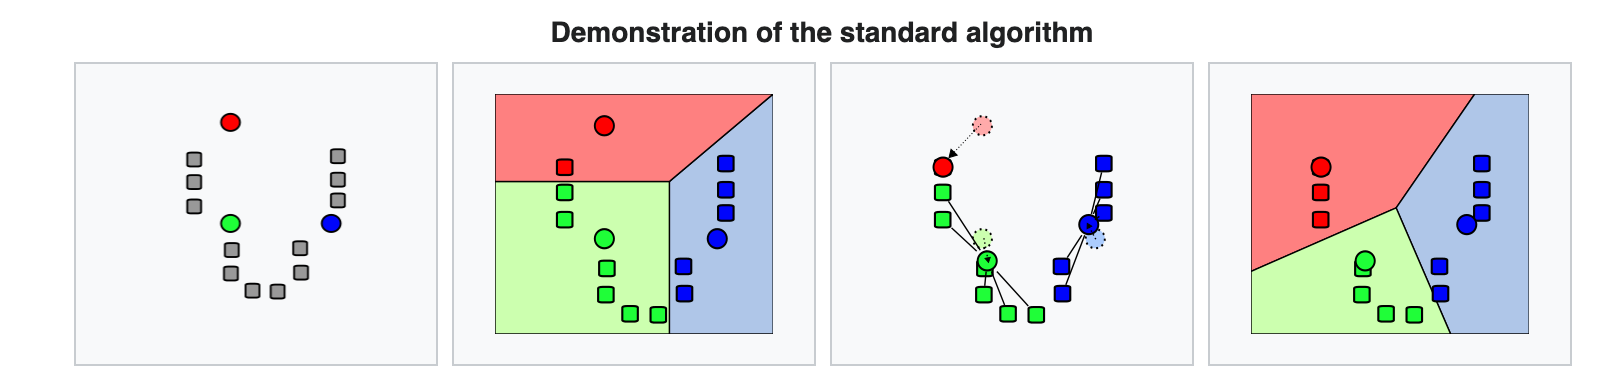
\includegraphics[width=10cm]{images/Kmeans.png}
    \caption[Iterations in K-means clustering]{Iterations in K-means clustering.\footnote{Source: https://en.wikipedia.org/wiki/K-means-clustering}}
    \label{Kmeans}
\end{figure}




\section{Experiments and results}
What follows are the optimal CT-model parameters, for the task of detecting shots in logs, and the experiments used to identify them. 

\subsection{Number of rays, angles and resolution} 

Something wise\footnote{See \url{https://drive.google.com/drive/folders/1LJ_m7pny6Ikl0HH2YcMOjl5B7i967D1S?usp=sharing}}

\subsection{Energy usage}\label{sec:energy-usage}
Based on the data described in section \ref{NISTDATA} we created the following plots (Figure \ref{fig:both-attenuation-coeff-plots}).
\begin{figure}[H]
    \centering
    \large{Attenuation coefficients} \\
    \begin{subfigure}[b]{0.32\textwidth}
        \centering
        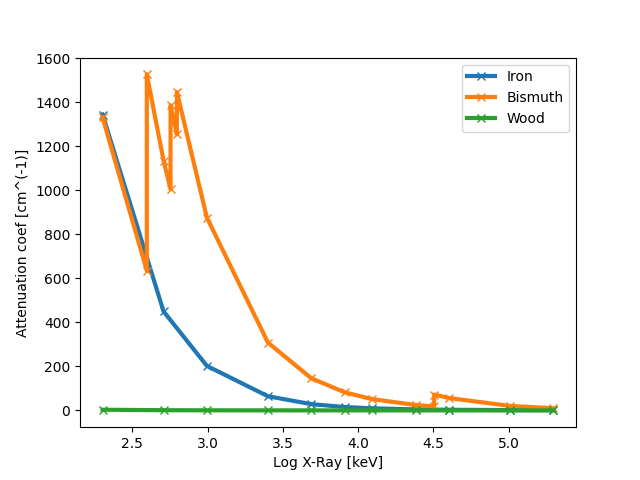
\includegraphics[scale=0.4]{images/attenuation_coef_zoom.png}
        \caption{\small Note that the x-axis is log scaled. Each mark on the graph is a data point from NIST. \newline}
        \label{fig:attenuation-coef-zoom}
    \end{subfigure}
    \begin{subfigure}[b]{0.32\textwidth}
        \centering
        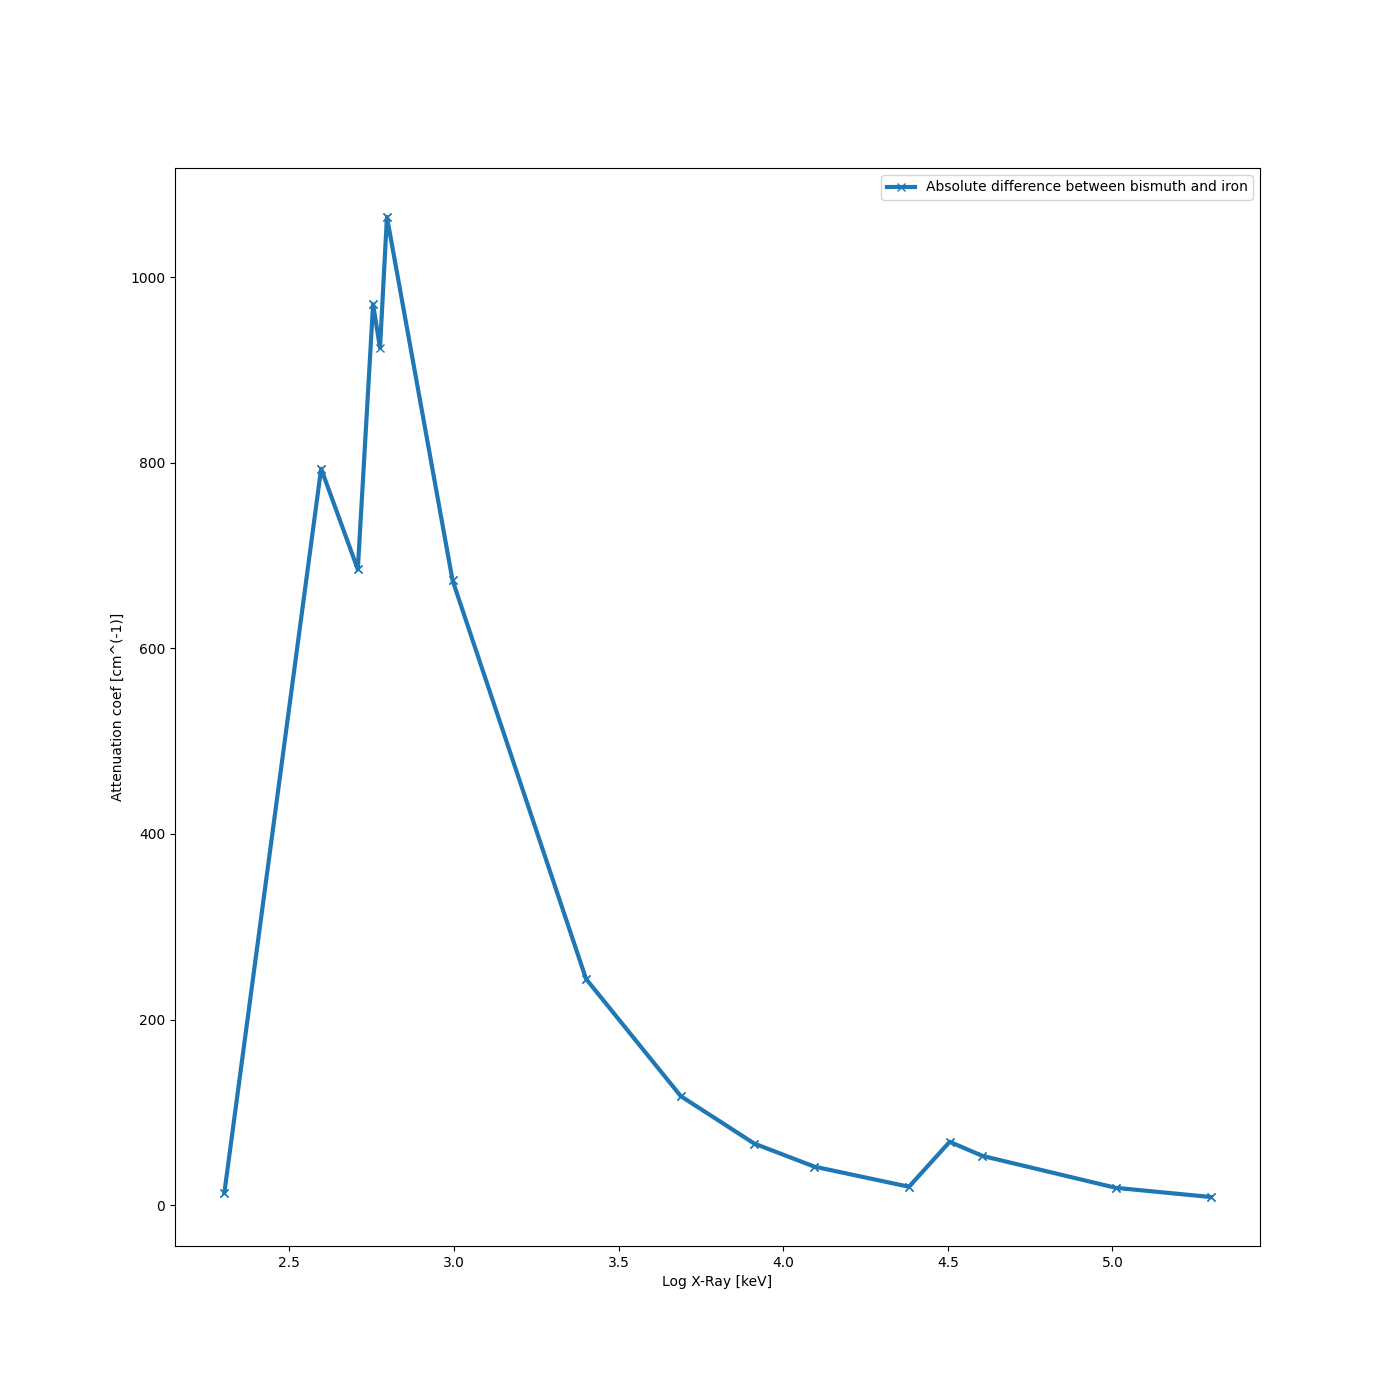
\includegraphics[scale=0.4]{images/diff-attenuation-coef-bismuth-iron-zoom.png}
        \caption{\small Absolute difference between the attenuation coefficients for bismuth and iron. Data is calculated using linear interpolation - see appendix \ref{appendix:attenuation-coefficients}.}
        \label{fig:diff-attenuation-coef-bismuth-iron}
    \end{subfigure}
    \begin{subfigure}[b]{0.32\textwidth}
        \centering
        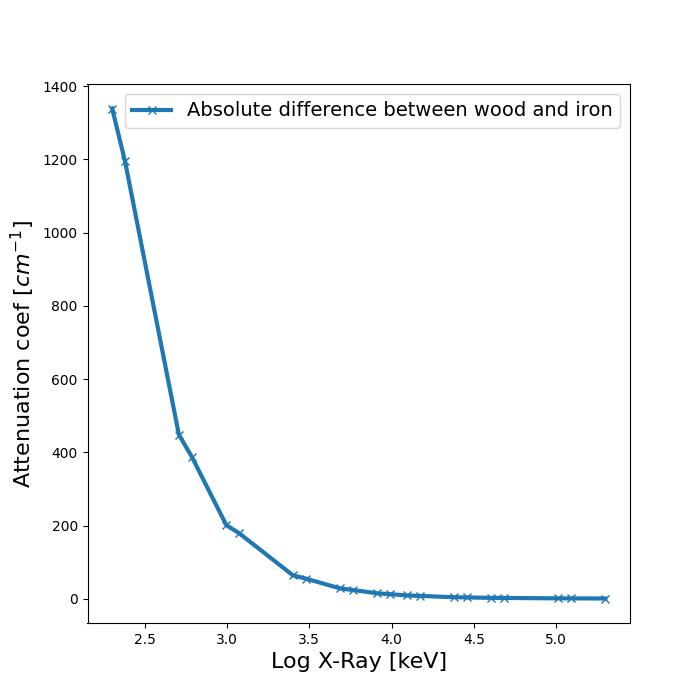
\includegraphics[scale=0.4]{images/diff-attenuation-coef-wood-iron-zoom.png}
        \caption{\small Absolute difference between the attenuation coefficients for wood and iron. Data is calculated using linear interpolation - see appendix \ref{appendix:attenuation-coefficients}.}
        \label{fig:diff-attenuation-coef-wood-iron}
    \end{subfigure}
    \caption{\small Note that in both of these images that they are only plotted in the log interval for commercial X-Ray (10 keV - 200 keV).}
    \label{fig:both-attenuation-coeff-plots}
\end{figure}

Based on Figure \ref{fig:attenuation-coef-zoom} and Figure \ref{fig:diff-attenuation-coef-bismuth-iron} we see that the best value for noticing a difference between wood, bismuth and iron is at 16.4 keV. 

Using Lambert Beer's law we also created the following plot which shows the ratio between input and output energy intensities depending on different energy levels (Figure \ref{fig:energy-vs-output-percentage}.). 

\begin{figure}[H]
    \centering
    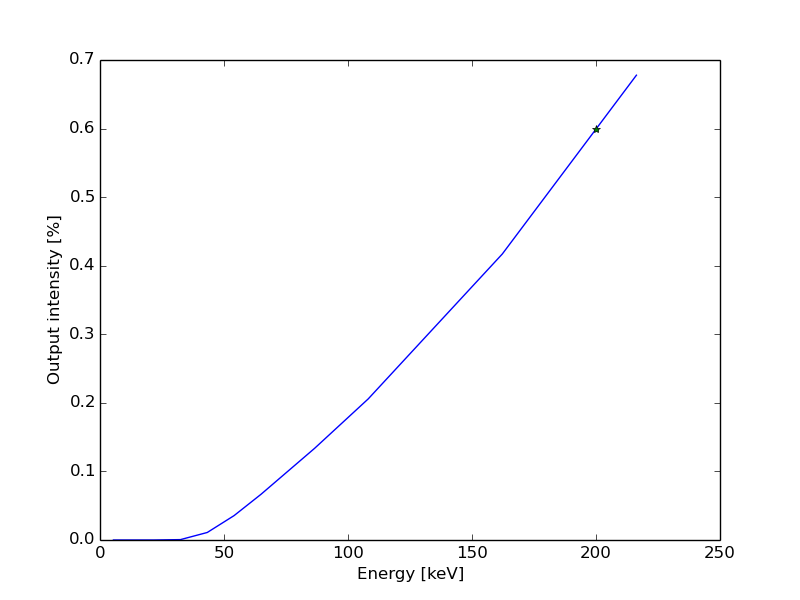
\includegraphics[scale=0.35]{images/energy-vs-output-percentage.png}
    \caption{The ratio between energy intensities as a function of the energy level measured in keV.}
    \label{fig:energy-vs-output-percentage}
\end{figure}

\section{Discussion}
To reconstruct an image from the attenuation distributions by a CT-scanner well enough to spot some detail, in this case shots in logs, there are a lot of parameters that can be tuned and approximations to be made. The specific approximations and simplifications to make is a model specific task and all come with tradeoffs.
???

% Bedre formuleringer for dette afsnit eksisterer helt klart
In Section \ref{sec:energy-usage} we saw that configuring the X-Ray to use 16.4 keV was the optimal energy level for differentiating between iron and bismuth using data from NIST. This however assumed that wood is completely homogeneous and therefore, before using the system in the "real" world, a better value could be found by trying different energy levels in a concrete example and then deciding on a value. 

\section{Conclude}
???

\section{The list ??? SKAL SLETTES}
\begin{itemize}
    \item Vinkler, rays, N osv. argumentation --> konditionstal + confusion matrix
    \item Ridge regression - test kvalitativ, confusion matrix og tid
    \item Skrive rapport og sætte alt pænt op
    \item References
    \item Gå gennem punkterne på peergrade og sikre, at alt er godt
    \item Assume normal distributions noise
    \item Discuss: Computational time 
    \item Downsampling and average in each block
\end{itemize}





\newpage
\appendix
\section{Mathematical derivations}
\subsection{Lambert Beer's Law}\label{appendix:lambert-beers-law}
If we consider Lamberts-Beer's law

\begin{equation}\label{eq:lamberts-beer}
    \diff{I}{\ell} = -x I(\ell),
\end{equation}

then, and assuming $I \neq 0$, we get

\begin{equation}
    \frac{I'(\ell)}{I(\ell)} = -x.
\end{equation}

Integrating both sides of this expressions yields

\begin{equation}
    \int_{0}^{\ell_{\max}} \frac{I'(\ell)}{I(\ell)} \; \mathrm{d}\ell = \int_{0}^{\ell_{\max}} -x \; \mathrm{d}\ell,
\end{equation}

so

\begin{equation}
    \ln{I(\ell)} \big|_{0}^{\ell_{\max}} = \int_{0}^{\ell_{\max}} -x \; \mathrm{d}\ell.
\end{equation}

Therefore by setting $I(0) = I_0$ and solving for $I(\ell_{\max}) = I$, which represents the intensity of the beam after it has passed through the sample, we get

\begin{equation}
    I = I_0 \exp{\left(-\int_{0}^{\ell_{\max}} x \; \mathrm{d}\ell \right)}.
\end{equation}

Or equivalently:

\begin{equation}
    \int_{0}^{\ell_{\max}}x \text{d} \ell = \log\left(\frac{I_0}{I}\right).
\end{equation}

As a special case when the material is homogeneous we get that $x = x_0$ is independent of $\ell$ and therefore

\begin{equation}
    I = I_0 \exp{(-x_0 \ell_{\max})}.
\end{equation}

% \subsection{Simplification of the model}\label{appendix:simplification-discreatization}
% Approximating the integral using the Riemann definition we get, using the given partition of $x_1, x_2, \dots, x_p$

% \begin{equation}
%     \int_{0}^{\ell_{\max}} x \; \mathrm{d}\ell \approx \sum_{j=1}^{p} x_j \ell_j.
% \end{equation}

\section{Code}
All code can also be found on GitHub \url{https://github.com/ElMiho/02526-exam-project}. 

\subsection{Exercise 1}
\subsubsection{With cvxpy}\label{appendix:exercise-1-cvxpy}
\lstinputlisting[language=Python, breaklines=true]{code/exercise_1_cvxpy.py}

\subsubsection{Without cvxpy}\label{appendix:exercise-1}
\lstinputlisting[language=Python, breaklines=true]{code/exercise_1.py}

\subsection{Attenuation coefficients}\label{appendix:attenuation-coefficients}
\lstinputlisting[language=Python, breaklines=true]{code/atttenuation_coef.py}

\subsection{Paralleltomo}\label{appendix:paralleltomo}
\lstinputlisting[language=Python, breaklines=true]{code/paralleltomo.py}

\subsection{Test functions}\label{appendix:generate-test-functions}
\lstinputlisting[language=Python, breaklines=true]{code/generate_test_functions.py}

\subsection{Ridge regularization}\label{appendix:ridge-regularization}
\lstinputlisting[language=Python, breaklines=true]{code/ridge_regularization.py}

\subsection{Validation}\label{appendix:validation}
\lstinputlisting[language=Python, breaklines=true]{code/validation.py}

\end{document}